\part{Theme \& Context}\label{ch:int}
  % Context - The Convolution operation
  Convolution is a mathematical operation that relates two signals into a third, representing how one is modified by the other. The operation forms the basis of impulse decomposition, and \citeonline{dsp_basic} described it as the most fundamental technique in Digital Signal Processing. More recently, the rapid growth of Convolutional Neural Networks (CNN) revolutionized the field of computer vision due to its high accuracy and ability to train over large sets of data~\cite{alzubaidi2021review}, further increasing the need to process convolution in modern computer systems.

  % Context - Constrained environments
  \textit{Resource- or Implementation-Constrained Environments} (referred to simply as ``constrained environments'' from this point on) are characterized by various limitations inherent to their hardware, software, or application. Examples include embedded, mobile or real-time applications, each with different designs and limitations. For instance, an embedded system is usually constrained regarding processing power and physical space, while a real-time application might have more processing power but is constrained regarding latency and throughput.
  
  % Context - Cloud computing
  Large-scale convolution, such as in most CNNs, is resource-intensive in terms of processing, memory, and power consumption~\cite{ujiie2016approximated}. Applications in constrained environments traditionally offload their processing load to external servers connected to the internet, in what is known as the \textit{Cloud Computing Paradigm}~\cite{rashid2019cloud}. However, this approach relies on how much data can be  \textit{communicated} over a period of time (bandwidth) rather than how much data can be \textit{processed} over a period of time (processing speed). Bandwidth does not scale as easily as processing speed, and can often present an issue in constrained environments.

  % Context - Cloud computing
  Another approach is installing intermediary systems closer to the application, which can process high workloads in real-time with low communication latency, storing large sets of sensitive data and mediating communication with the cloud. These systems became known as ``edge applications'' and form the core of the \textit{Edge Computing Paradigm}~\cite{cao2020overview}.
  
  % Examples
  The convolution process, individually or as part of a CNN, has seen many recent applications in constrained environments using tools such as edge computing. Examples include facial~\cite{khan2019deep} and emotional~\cite{zhang2019face} recognition, access authentication~\cite{xie2019convolution}, image processing~\cite{colbert2021energy} and cybersecurity~\cite{zhou2019lightweight}.
  
  % Present Theme
  Today, an active field of research focuses on optimizing specific-purpose architectures in terms of metrics relevant to constrained environments, which is the theme of this project. The traditionally studied metrics include latency, energy efficiency, and scalability. However, recent research~\cite{li2022hardware} has indicated the importance of a more targeted metric known as \textit{hardware efficiency}, measured as a ratio between latency and hardware resource utilization.
  
  % Segue and mention objective
  Next, in Chapter~\ref{ch:rev}, a literature review will be performed to explore the domain of this theme and reveal problems that are yet unsolved or partially unsolved and whose solution may contribute significantly to the field. These problems will form the foundation to state the objective of the project in Chapter~\ref{ch:obj}.

\part{Literature Review}\label{ch:rev}
  With regards to the optimization of convolution processing, several surveys have been performed concerning significant technological developments in this field. These include efficient algorithms~\cite{mittal2021survey}, hardware~\cite{feng2019computer}, platforms such as FPGAs~\cite{abdelouahab2018accelerating}, ASICs~\cite{moolchandani2021accelerating}, and overall optimizations~\cite{zhang2019recent}.
  
  Based on this body of work, Sections~\ref{sec:conv_alg}, \ref{sec:hard_acc}, and \ref{sec:plat} cover the relevant technological developments of convolution algorithms, hardware acceleration, and computer platforms, with an emphasis on viability in constrained environments.

  \chapter{Convolution Algorithms}\label{sec:conv_alg}
    Concerning hardware applications, three parameters can be used to describe the applicability of an algorithm:

    \begin{itemize}
      \item \textbf{Complexity}: Relating to the total number of \textit{elementary operations}\footnote{An \textit{elementary operation} is defined as a computing operation that takes a fixed amount of time to be processed by a particular computing machine. Consequentially, the set of elementary operations used for complexity analysis depends on the model of computation used, as different abstract and physical machines will have widely different sets of instructions. For the purposes of fair comparison between different architectures, this project will refer to any \textit{single-bit arithmetic or logical operations} as elementary operations.}
      that must be performed to complete the task. This factor, while important, is not the only determinant of hardware efficiency.
      
      \item \textbf{Parallelization}: Independent operations can be performed simultaneously in hardware, given sufficient memory and components. An algorithm with many independent operations might still be faster than a more complex one with more dependencies.
      
      \item \textbf{Memory Footprint}: Some computational processes require more buffer memory to store variables currently in use. If the memory used by the algorithm is larger than the available cache, the processor has to store and load from outside the chip, leading to slowdown. Domain-specific architectures usually contain just enough memory for their core processes.
    \end{itemize}

    \section{Convolution-over-space \& Matrix Multiplication}
      Signal convolution over sets of Euclidean-organized data (e.g., arrays, images) can be represented by the ``sliding product'' of two inputs. The filter (or \textit{kernel}) ``slides'' across the input, multiplying each pair of coincident points and adding the products together. Each of these results represents a convolution centered on a different input point. All of them are organized jointly as the output of the convolution. In image processing, we refer to this operation as ``convolution-over-space''.
  
      The output can have varying sizes depending on how we handle the sliding of the kernel out-of-bounds~\cite{alzubaidi2021review}:
  
      \begin{itemize}
        \item If we ignore every position of the kernel in which any of its points coincide with out-of-bounds data: the output size is smaller, proportional to the kernel's size, and referred to as \textit{valid} convolution.
          
        \item If we require only the center point of the kernel to coincide with valid data and the out-of-bounds data equal to zero: the output size is the same as the input, referred to as \textit{same} convolution.
          
        \item If we consider every position of the kernel that coincides with at least one valid point of data and the out-of-bounds data equal to zero: the output size is larger, proportional to the kernel's size, and is referred to as \textit{full} convolution.
      \end{itemize}
  
      Let $s$ be the size of the output of a single-dimension full convolution such that $s = p + k - 1$, where $p$ is the dimension of the input, and $k$ is the dimension of the kernel. The number of multiplication operations required by convolution-over-space is $M_{op} = ks$. 
    
      This can be expanded to higher dimensions, in which the number of multiplications equals the input's total size times the kernel's total size.
  
      It is possible to arrange the input and kernel into matrices such that their matrix multiplication becomes equivalent to their convolution~\cite{vasudevan2017parallel}. Naive matrix multiplication does not reduce the complexity of the algorithm but does allow for a parallelization technique detailed in Section~\ref{sec:systolic}.
      
      The mathematical convenience of matrix multiplication and lack of transformations makes this method simple to process on conventional hardware, making it the standard for CNN convolution processing~\cite{zhou2021characterizing}.

    \section{Coppersmith-Winograd}
      An open problem in modern mathematics is finding the smallest $\omega$ such that the number of operations required by an $N \times N$ matrix multiplication equals $N^{\omega + O(1)}$~\cite{gao2020systematic}. The naive line-by-column multiplication method has $\omega = 3$, and the current lowest known value for $\omega$ is 2.37188~\cite{duan2022faster} using a method based on the Coppersmith-Winograd algorithm, which is currently the state-of-the-art in terms of speed~\cite{lavin2016fast}.
        
      The Coppersmith-Winograd algorithm samples the input and kernel at a given set of points using transform matrices so that their Hadamard product (element-wise multiplication), followed by the respective inverse transform, equates the convolution of the original signals. This method becomes inefficient for larger kernels, so smaller kernels (e.g., 3x3 or 5x5) are most often used~\cite{alam2022winograd}.

      The requirement for small kernels is convenient, considering modern CNNs tend to have many layers with small filters, such as MobileNetV2~\cite{sandler2018mobilenetv2}. However, the deeper layers of these networks use a large number of filters, which act as a third dimension of convolution. MobileNetV2 can reach a depth of 960 in the later layers, turning a 3x3 convolution into a 3x3x960 convolution and severely impairing the Coppersmith-Winograd method.
      
      The standard approach is to divide the input into small blocks and convolve each with the kernel. Coppersmith-Winograd computes multiple outputs simultaneously, converting any available parallelism opportunity into speed. As the input block size \textit{increases}, the number of multiplications required by the Hadamard product \textit{decreases} to a theoretical minimum of $s$~\cite{barabasz2020error}. However, the number of additions and constant multiplications required by the transform also increases exponentially, making this method is more suited for applications requiring fewer transforms~\cite{zlateski2019anatomy}.
      
      Additionally, increasing input block size increases the floating-point error exponentially~\cite{alam2022winograd}. Hence the method incurs an inherent trade-off between speed and precision that must be accounted for.

    \section{FFT Convolution}
      The Theorem of Convolution defines the operation as follows:
    
      \begin{equation}
        [g * h](x) \Leftrightarrow F^{-1}[G \circ H](y),
      \end{equation}
        
      \noindent where $G$ and $H$ are the \textit{Fourier Transforms} of the respective signals $g$ and $h$; $F^{-1}$ is the \textit{Inverse Fourier Transform}; $*$ denotes convolution; $\circ$ denotes the Hadamard product (pointwise product); $x$ denotes an arbitrary domain and $y$ denotes the respective Fourier domain of $x$.
      
      The theorem states that signal convolution in a particular domain is equivalent to pointwise multiplication in its Fourier domain. This allows us to compute convolution by calculating the Discrete Fourier Transform (DFT) of the input and kernel in the domain of space (represented by $ \sigma$), applying the Hadamard product in the respective Fourier domain of space (represented by $\zeta$), and then calculating the Inverse Discrete Fourier Transform (IDFT) as such:
        
      \begin{equation}
        [p * k](\sigma) = F^{-1}[F(p) \circ F(k)](\zeta)
      \end{equation}          
  
      The traditional DFT (matrix multiplication between the signal and a twiddle factor matrix) has complexity $O(s^2)$. Instead, we can use the Fast Fourier Transform (FFT) algorithm, which exploits the symmetry in the Fourier Transform and has complexity $O(s\log_2s)$. The same relationship applies to the IDFT and IFFT (Inverse Fast Fourier Transform).
  
      The FFT convolution, therefore, scales almost linearly with the size of the image. It does \textit{not} scale directly with the size of the kernel, as does the matrix multiplication method. This fact was shown to significantly increase processing speed when using larger kernels~\cite{jha2007ieee}.
  
      Furthermore, it is possible to subdivide the input into kernel-sized pieces, perform FFT convolution in each one, and add the overlapping values, resulting in the full convolution of the undivided input~\cite{highlander2016very}. This method, known as \textit{overlap-add}, reduces the asymptotic complexity of the operation to $O(s\log_2k)$.
  
      However, the arrays transformed by the FFT are in the \textit{Complex Domain}\footnote{Whenever the word ``complex'' refers to the Complex Domain ($\mathbb{C}$), we shall capitalize it to differentiate it from the concept of \textit{complexity} used in other parts of the text, for the sake of cohesion. Similarly, the word ``real'' will be capitalized when referring to the Real Domain ($\mathbb{R}$).\\} %
      and thus require Complex operations. Most prominently, the Hadamard product becomes a series of Complex products, which are usually calculated as four Real products and two additions but can be simplified to three Real products using a less-known method\footnote{$(x_0+ix_1) = [x_0y_0-x_1y_1,i(x_0y_1+x_1y_0)] = [u_cv_a-u_av_c,i(u_av_c+u_bv_b)]$,\\where $u_a=x_0;v_a=y_0;u_b=x_0+x_1;v_b=y_1;u_c=x_1-x_0;v_c=y_0+y_1$~\cite{lavin2016fast}}. %
      Regardless, the Complex product can drastically increase computational requirements depending on the hardware used.
  
      Instead, we can employ the polar representation of Complex numbers in which multiplication is equivalent to one Real multiplication (the amplitude) and one Real addition (the phase), as such:
      
      \begin{equation}\label{eq:Cmult}
        A\phase{\alpha_1} \cdot B\phase{\alpha_2} = AB\phase{\alpha_1+\alpha_2}
      \end{equation}
  
      This method incurs the downside of requiring trigonometric operations, but there exist algorithms that can efficiently process these operations, as described in Section~\ref{sec:cordic}.

    \section{Comparison}
      On a purely mathematical complexity analysis, the Coppersmith-Winograd algorithm has the potential to reach $s$ multiplications in the Hadamard operation. However, its transform still scales exponentially with $s$. In contrast, the Fast Fourier Transform and its inverse have complexity $O(s\log_2s)$, and the Hadamard operation also has $s$ multiplications, albeit in the Complex realm. In addition, the FFT method can benefit from overlap-add, effectively lowering its complexity to $O(s\log_2k)$.
  
      The standard matrix multiplication algorithm with $ks$ multiplications has the highest potential for parallelization, as every multiplication is independent. It is usually processed as an $n \times n$ matrix multiplication resulting in $n^3$ multiplications. Accelerators such as Google's Tensor Processing Unit (TPU)~\cite{jouppi2020domain} leverage this potential in a systolic array architecture, lowering the system's overall latency, but become subject to hardware and power limitations as described in Section~\ref{sec:systolic}. Coppersmith-Winograd and the FFT methods share the ability to parallelize their Hadamard multiplications and parts of their transforms.
  
      Finally, regarding memory footprint, the FFT method has a higher memory requirement than Coppersmith-Winograd, due in part to its Complex operations~\cite{lavin2016fast}.

  \chapter{Hardware Acceleration}\label{sec:hard_acc}
    A large and accrescent amount of hardware acceleration technologies has been developed for applications in modern processors. Here, we will narrow our focus to technologies that have recently succeeded in accelerating convolution algorithms.

    \section{Systolic Array}\label{sec:systolic}
      First described in 1979 as a specific-purpose VLSI system~\cite{kung1979systolic}, systolic arrays have re-appeared as a core feature of some modern low-latency implementations such as Google's TPU. A systolic array is a topological assortment of processing units commonly referred to as \textit{nodes}. Each node is designed to process fractions of the desired operation and send information to each neighbor, forming a \textit{stream} that eventually leads to a complete operation. In particular, the input of the systolic array can be shared between nodes, removing the need to re-read the input value from a register. As such, computationally complex operations can be subdivided and performed within fewer machine cycles.
          
      However, to maintain its low latency, the size of a systolic array has to grow at the same rate as the complexity of the target operation. For example, consider the convolution of a 256x256 black-and-white image with a 4x4 kernel. Using the TPU's matrix multiplication systolic array, which contains 65536 multiply-and-add nodes, the operation can be completed within exactly 16 cycles. In order to process a 512x512 image in the same number of cycles, the systolic array would now require four times as many nodes, totaling 262144.
      
      This exponential increase in hardware requirements reduces the application's viability in constrained environments. Likewise, if the complexity of the target operation scales at a slower rate, so do the hardware requirements of the systolic array.

    \section{CORDIC}\label{sec:cordic}
      Coordinate Rotation Digital Computer (CORDIC) is an algorithm initially conceptualized in 1956 and later developed into an iterative algorithm capable of fast, low-cost computation of various mathematical functions~\cite{meher200950}.
      
      \begin{figure}[htb]
        \caption{Quintessential CORDIC Block Diagram}
        \centering
        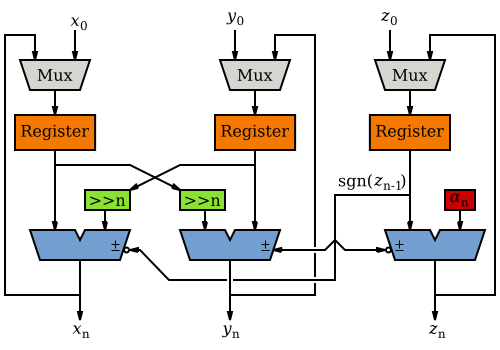
\includegraphics[width=\textwidth]{figures/cordic.pdf}
        %\legend{Source: Public domain~\cite{wikimedia_cordic}}
        \todo{figure out how to add sources to images}
        \label{fig:cordic}
      \end{figure}
  
      As shown in Figure~\ref{fig:cordic}, a simple CORDIC implementation requires only elementary operations and a small number of components. Despite this, it can be used to perform mathematically complex operations within a fixed number of cycles. The fully asynchronous system of Figure~\ref{fig:cordic} calculates one iteration of the CORDIC algorithm per cycle and can thus be re-utilized as part of its iterative process to increase hardware efficiency further.
  
      The standard algorithm known as \textit{Unified CORDIC} is capable of calculating arbitrary vector rotation in circular, linear, or hyperbolic coordinates. Each iteration approaches the expected result with a precision of $2^{-j}$, where $j$ is the number of iterations. As such, for complete precision, its complexity is $O(n)$, where $n$ is the number of bits~\cite{meher200950}.
      
      For the purposes of FFT convolution, CORDIC is capable of converting Complex numbers from rectangular to polar coordinates. Thus, to multiply two Complex numbers, we can convert both to polar coordinates using CORDIC, multiply them as polar coordinates, and convert them back. This process allows the calculation of Complex multiplication with one Real multiplication and one Real addition, as demonstrated in Equation~\ref{eq:Cmult}.
      
      Modern CORDIC implementations build upon the design of Unified CORDIC in various ways, such as processing multiple CORDIC blocks in parallel (known as ``Radix-$X$ CORDIC'', where $X$ is the number of parallel blocks), pre-processing input data, and pre-calculating trigonometric operations of chosen angles~\cite{sharmareview}. These optimizations are often application-specific or incur considerable downsides. Higher-radix CORDIC, for instance, reduces latency by increasing hardware usage at the same rate. For our project, a modified single-Radix Unified CORDIC implementation is used. This is due to a method of calculating Complex multiplication concurrently using the Karatsuba algorithm, detailed in Section~\ref{sec:flux}.
    
    \section{Efficient Multiplication}
      Multiplication is the most demanding operation in all convolution algorithms described in this review. Hence why the algorithms presented often focus on reducing the total number of multiplication necessary for convolution. A complementary approach is to reduce the complexity of the multiplication operation itself.
  
      We will focus on fixed-point multiplication, as neural network implementations have been shown not to require the extra precision of floating-point numbers~\cite{courbariaux2014training}.
  
      For two arbitrary $n$-bit integers (or otherwise fixed-point numbers), the classical long multiplication has complexity $O(n^2)$, and the hardware required by a naive implementation of this algorithm also grows quadratically. Lower asymptotic bounds have been achieved with the Karatsuba~\cite{karatsuba1962multiplication}, Toom–3~\cite{wang2000explicit}, Schönhage–Strassen~\cite{schonhage1971fast}, and Harvey-Hoeven~\cite{harvey2021integer} algorithms. The latter is conjectured to have reached the lowest possible asymptotic bound for this problem: $O(n\log_2n)$. However, these algorithms require increasingly large input values to become efficient outside of asymptotic analysis. Harvey-Hoeven is theorized to become efficient for inputs of roughly $10^{86}$ digits.
      
      The Karatsuba algorithm is estimated to be faster than long multiplication at about 128 bits~\cite{machhout2008efficient}, which is much lower than the number of bits required by the other algorithms mentioned. Karatsuba is a particular case of the Toom-Cook algorithm and is technically referred to as Toom-2. It is a divide-and-conquer algorithm capable of recursively subdividing an $n$-bit fixed-point multiplication into a maximum of $n^{\log_23}$ single-bit multiplications, hence $O(n^{\log_23}) \approx O(n^{1.58496\ldots})$. Critically, this allows for each single-bit multiplication to be processed independently, leading to a trade-off between the algorithm's increased complexity for smaller inputs and its potential for parallelism. If preceded by a CORDIC system, this property allows for the the calculation of each single-bit multiplication concurrently with each CORDIC cycle, as detailed in Section~\ref{sec:design}.
      
      Also of note, a convolution algorithm for CNNs without multiplications has been develop using CORDIC exclusivelly~\cite{parmar2019resource}. However, their implementation relies on a quirk of the Max Pooling layer that allows re-scaling of the input variables. This approach, therefore, limits the algorithm to specific CNN topologies that include a Max Pooling layer preceding a convolution layer. Moreover, while the implementation is hardware-efficient, its latency falls short of other state-of-the-art implementations that rely on multiplication.
  
  \chapter{Platforms}\label{sec:plat}
    \section{General \& Specific Purpose}
      General purpose architectures (commonly CPUs) are sometimes used for specialized processing, depending on the application, but are overall less efficient than GPUs and other specific-purpose architectures~\cite{chen2019deep}. CPUs are generally not optimal for CNN processing~\cite{hu2022survey}.
  
      In contrast, Application Specific Integrated Circuits (ASIC) can, in theory, better utilize efficient algorithms and parallelization techniques, depending on how specialized the design is for that application. The Graphic Processing Unit (GPU), one of the most widespread co-processors, is often used for machine learning applications due in part to its availability. More specialized ASICs can achieve higher performance and energy efficiency at the cost of versatility~\cite{hu2022survey}.

    \section{FPGA}
      Field-Programmable Gate Array (FPGA) is a versatile platform capable of describing efficient re-programmable computer architectures. It is valued for its high energy efficiency, scalability, parallelization potential, and versatility in implementation. These advantages can facilitate the quick deployment of low-latency processors, which is advantageous in constrained environments requiring periodic hardware updates, such as ~\citeonline{garvey2003use}.
      
      FPGAs also had substantial disadvantages which have been addressed over time as the technology gained popularity. \citeonline{maclean2005evaluation} described the three major disadvantages of FPGA implementation as: inefficient floating-point arithmetic, high overhead leading to large device sizes, and a challenging design process. Since then, FPGAs have shown state-of-the-art efficiency in floating point arithmetic~\cite{lian2019high}~\cite{de2022fast}; low overhead implementations~\cite{zhou2019fpga}, including FFT implementations~\cite{wang2020low}; and more streamlined design processes~\cite{haris2021secda}.
  
      Due to an ongoing research and development process for FPGA technologies, it has steadily developed into an efficient platform for time-critical and energy-efficient systems~\cite{ullah2020energy}, including edge applications~\cite{biookaghazadeh2018fpgas}.

\part{Objective}\label{ch:obj}
  Based on the literature review performed, we can now choose a target problem. We can then hypothesize a solution to the problem and justify it, thus composing a verisimilar conjecture. Only then can we determine our objective and expect to contribute significantly to our field by accomplishing it.

  \chapter{Target Problems}\label{src:prob}
    When choosing an algorithm, its complexity is the most closely related metric to hardware efficiency. While parallelization can vastly improve latency, it does not affect the raw number of operations required to complete the algorithm. This exposes a problem in systolic array matrix multiplication implementations, such as Google's TPU. While the inherent parallelism of the application can lead to extremely low latencies, the number of components scales quadratically with the input size. In other words, the speed gain provided by a single component, i.e., its \textit{hardware efficiency}, also decreases quadratically.

    Furthermore, edge applications, which can amortize the processing load on constrained systems, benefit from scalability and adaptability to changes in demand~\cite{ferrer2019towards}. Scalability, in turn, becomes more viable when the impact of each component is higher.

    state-of-the-art accelerators are commonly implemented in ASIC technology to benefit from modularity. However, in specific-purpose-constrained implementations, the unchangeable nature of ASICs can become an expensive rigidity in the design. Programmable devices and FPGAs are more capable of versatility, scalability, and adaptability.
  
  \chapter{Hypothesis \& Justification}\label{src:hyp}
    Our review shows that the FFT convolution algorithm can be employed with almost linear complexity, while the standard matrix multiplication algorithm has quadratic complexity. Both methods are highly parallelizable and do not incur a significantly high memory footprint. The main disadvantage of the FFT method is the required use of Complex multiplication, which usually requires over three times more operations than Real multiplication and is not optimized by most processors. This disadvantage, however, can be amortized by employing the CORDIC algorithm in FPGA technology.

    % Hypothesis
    Thus, we hypothesize that higher hardware efficiency can be achieved while maintaining real-time latency by way of a new convolution-specialized architecture, consisting of a CORDIC-augmented FFT convolution algorithm and its implementation in a highly versatile and parallelizable FPGA environment.

    % Justification
    Such an implementation should achieve similar or linearly lower latency to matrix multiplication while exponentially decreasing hardware and power requirements. This is justified by the algorithm's linear growth of complexity, linear growth of components, and the FPGA's inherent energy efficiency.

    % Objective
    The primary objective of this project is to verify whether a CORDIC-augmented FFT convolution accelerator can surpass state-of-the-art hardware efficiency. The implementation will be designed and evaluated against the established systolic array matrix multiplication architecture.
    
    %The objective of this project is to verify whether such an implementation can surpass state-of-the-art hardware efficiency.
    
    %The objective of this project is to confirm the viability of an FFT convolution accelerator as a hardware-efficient alternative to the state-of-the-art matrix multiplication accelerators.
    
    %demonstrate, through this implementation, 
    % This demonstration will be carried out by implementing and testing an especially-designed architecture under these paradigms.
  
\part{Method}\label{ch:met}
  Our method consists of designing the conjectured architecture, implementing it, and testing it against recognized benchmarks.

  \chapter{Benchmarks}\label{sec:bench}
    \todo{[...]}

  \chapter{Architecture Design}\label{sec:design}
    The central idea of the design is to augment an FFT convolution algorithm using rectangular-polar and polar-rectangular conversions to simplify Complex multiplication, as shown in Figure~\ref{fig:dataflow}. The rectangular-polar conversion can be efficiently processed with CORDIC in \textit{Vectorization} mode, and the polar-rectangular conversion in \textit{Rotation} mode.
    
    \begin{figure}[htb]
      \caption{High-level diagram of the FFT-CORDIC convolution algorithm developed.}
      \centering
      
\includegraphics{figures/dataflow.png}
      %\legend{Source: authors}
      \label{fig:dataflow}
    \end{figure}

    In Figure~\ref{fig:dataflow}, $R\left [ N \right ]$ are the input and kernel arrays of $N$ Real numbers, $C_p\left [ 2N \right ]$ are arrays of $2N$ Complex numbers in \textit{polar} coordinates, $C_r\left [ 2N \right ]$ is an array of $2N$ Complex numbers in \textit{rectangular} coordinates, and $R\left [ 2N \right ]$ is the output array of $2N$ Real numbers.

    This simple design will be enhanced and optimized in the following sections, leading to the parallelism and hardware efficiency required by the objective.

    \section{General Specifications}
      Internally, the architecture uses 16-bit \textit{unsigned integers}. There are two reasons for this choice. First, the binary representation of these numbers is equal to the value they represent, allowing the use of some useful binary properties, most prominently the equivalence between bit-shifting and multiplication by powers of 2. Second, while the use of double-precision floating-point variables in convolution is common, particularly in CNNs, due in part to the ability of modern CPUs and GPUs to process floating-point numbers \textit{en masse}, CNNs are not significantly affected by low precision operations~\cite{courbariaux2014training}.

      %When signed integers are necessary, the sign-bit will be kept independent from the unsigned integer to preserve the binary properties.

      An $n$-bit multiplier usually requires a $2n$ buffer to store full precision. As stated, full precision is not required, but as our initial bit precision is already low at 16, we will use a full 32-bit buffer.

      The input and kernel arrays must also be padded with zeroes to $2N$ to prevent cyclic convolution. However, in the Complex Domain, \textit{hermitian symmetry} guarantees that $N-1$ out of the $2N$ elements of the array are the Complex conjugates of other elements, making them redundant. In practice, the hardware will be designed to calculate only the non-redundant values and then abstract the redundant values by simply fetching the equivalent element and changing its Complex sign-bit.
        
    \section{The Flux Multiplier}\label{sec:flux}
      \todo{Consider removing this entirely}

      The major contributor to parallelization in our design is the \textit{Flux Multiplier}, which allows the computation of the multiplication step concurrently with both rectangular-to-polar CORDIC transforms.
      
      Recall from Section~\ref{sec:cordic} that each CORDIC iteration approaches the expected result with a precision of $2^{-j}$, where $j$ is the number of iterations. This means that after the first cycle, the most significant bit is almost certainly correct, except for a possible future bit-carry, which is unlikely due to the converging nature of the algorithm\footnote{The probability of a bit-carry affecting the correctness of the algorithm will be measured experimentally at the simulation stage, but is expected to be insignificant. If correctness is an issue, an asynchronous reset can be implemented to restart the process in the event of a bit-carry.}.
      Effectively, the system receives one bit each from the two vectorization-mode CORDICs every cycle, which it can use to calculate the multiplication concurrently using a variant of the Karatsuba algorithm described below.
      
      Let $A$ and $B$ be $n$-bit fixed-point numbers, and $C$ be a $2n$-bit fixed-point number such that $C = AB$. If we know a certain amount of most significant bits of $A$ and $B$ and receive a new one ($A'$, $B'$), we can add the new bit into the known number by shifting the known number to the left once (equivalent to multiplication by 2 in binary) and adding the new bit. This gives us an iterative multiplication process, with $t$ as the iteration number:
      \begin{equation}
          C_{t+1} = (2A_t + A')(2B_t + B')
      \end{equation}
      
      Expanding this product, we have:
      \begin{equation}
          (2A_t + A')(2B_t + B') = 4A_tB_t + 2A_tB' + 2B_tA' + A'B'
      \end{equation}
      
      We can then apply the following simplifications: $A_tB_t = C_t$; the multiplication operations with $A'$ and $B'$ are binary operations and therefore equivalent to AND (represented by $\land$); multiplication by 2 or 4 is equivalent in fixed-point arithmetic to shifting (represented by $x \ll y$, where $y$ is the number of shifts). This leads us to the final equation:
      \begin{equation}
          C_{t+1} = [C_t \ll 2] + [(A_t \land B') \ll 1] + [(B_t \land A') \ll 1] + [A' \land B'],
      \end{equation}
      which is composed solely of logical AND operations, non-variable shifts, and additions. In hardware, these operations can be executed in extremely fast and efficient instructions compared to multiplication.

    \section{Design Integration}
      \todo{[...]}
      
  \chapter{Synthesis \& Testing}\label{sec:synth_test}
    \todo{Update. Maybe split into two chapters}

      Each part of the design will be described in Verilog and integrated with System Verilog. The final design will be synthesized and simulated using open-source software for the sake of speed during initial debugging. For on-board testing, the respective proprietary software will be used to re-synthesize the project into the chosen technology.

      Based on our review, we have selected five metrics to be measured during testing. They are: Component utilization, number of cycles, latency, power consumption and precision. The first three are required to measure hardware efficiency, power consumption is relevant for constrained systems, and precision is used to evaluate correctness. To cover each of these metrics accurately, we have to run two kinds of tests: software simulations and on-board tests.

      Component utilization in FPGA technology can be measured generically in lookup tables (LUTs) usage, which constitute the greater part of a logic cell. However, many, if not most, of the operations required by convolution can be offloaded to DSP blocks found in most FPGA architectures. Therefore, two measurements will be made: the design synthesized with only LUTs and the design synthesized with as many DSPs as feasible without altering the functionality of the design. They can both, however, be performed during software simulation.

      The number of cycles is independent of the technology used. It varies with input size (as do all other metrics), but it is \textit{not} agnostic to input value. Some edge cases may cause an asynchronous reset, increasing the total number of cycles.

      The overall latency of the implementation depends on more than just the architecture design (e.g., central processor delay, fiber latency, overhead). However, it provides a more realistic measure of hardware efficiency.

      Power consumption is more straightforward and can be measured during software and on-board simulations. The on-board simulation is more precise but requires more setup, as described in the following section about testing procedures.

      Finally, the algorithm's precision does not depend on the technology used; unless the technology has some inherent precision loss or architectural choices that forfeit correctness for speed. It can be measured during software simulation and used as a debugging tool. The algorithm's precision will not be complete due to type conversions and other minor inaccuracies. However, we do not expect these inaccuracies to distort the result significantly.

      \section{Testing Procedures}
        \begin{itemize}
          \item \textbf{Random Arrays}: The system will process random input and kernel arrays, and their convolution will also be calculated externally with full precision. The result from the system should be coherent with the external calculation, ensuring the operation's correctness. The system's precision can be measured based on the results' differences. The number of cycles and component utilization can also be extracted from this test, as it is done in software.
          
          \item \textbf{Edge-case Analysis}: Extremely large or small arrays will be chosen in order to observe whether the system behaves as expected within these cases. This test does not provide any new metric, but it ensures the correctness of the algorithm.
          
          \item \textbf{Latency Testing}: A simple on-board setup will be assembled, and the real processing time of the circuit will be measured by considering factors such as overhead.
          
          \item \textbf{Power Measurement}: The board's power cable will be connected to a finely-controlled source, and different routines will be run to measure the energy consumption differential.
        \end{itemize}

\part{Results}\label{ch:res}
  \todo{[...]}

\part{Conclusions}\label{ch:con}
  \todo{[...]}
















% This block of text is just leftover, but I'll leave it here in case I can use it later

  % A standard CORDIC implementation takes $n$ cycles to finish processing, where $n$ is the fixed-point bit size of each input. Note the distinction between $n$ and $N$, the number of points in the FFT, which is assumed the same for the input and kernel due to the existence of the overlap-add method.

  % Naively, using a longhand multiplier, the algorithm's total number of cycles spent can be estimated at $2N(n^2 + 2n) + 2\log_2(2N)$. Traditional convolution spends about $N^2n^2$ cycles, which is asymptotically slower but more straightforward and efficient in most practical cases. However, the FFT algorithm is much more flexible in how we approach its processing and parallelization. We can employ several algorithmic and hardware-level optimizations to reduce the required number of cycles without significantly increasing the number of components. We will describe several such optimizations in the following sections.

  % As a practical benchmark for later comparison, let us consider a massively parallel traditional convolution architecture. A systolic array can process several fused multiply-add (FMA) operations per cycle, depending predominantly on the number of components used. The algorithm requires (in single-dimension, for simplicity) approximately $N^2$ MAC operations. If we desire to run X operations in a single cycle, we require X $n$-bit FMA cores. A floating-point 16-bit FMA core in FPGA uses --- components, therefore ... 
  % The design decisions made from this point onward in our project focus on improving this ratio.

  % % Perhaps I can just mention how this can use DSPs or ALMs and so on. We'll make a table later.